\chapter{Experiment}
\label{cha:Experiment}
This section describes the experiments conducted in order to be able, to answer the defined research questions. In the previous chapter (\ref{cha:Approach}) the general methodology used technologies got described, to gain an understanding of the implementation and its components. Based on this knowledge and implementation, some experiments got conducted, that provide interesting results and meaningful insights into this approach of neural audio synthesis. For the purpose of this thesis, some research questions have been defined, for which the following experiments, deliver the answers, which get discussed later on when showing the results.\\

\noindent Those research question are defined as the following:

\begin{itemize}
    \item \textbf{Is it possible to create novel sounds based on the characteristics of two instruments, by using ML technologies such as convolutional neural networks?}

    \item How do the pre processing steps influence the quality of the training, but also the quality of the output?

    \item How does the configuration/composition of a neural network influence the quality of the output?

    \item What are the information that are learnt from the neural network?

    \item By using audio spectrograms, are they suited best to achieve this task?
\end{itemize}

In the last section, when describing the different technologies, it has been mentioned, that they can be parameterized in order to influence the outcome of this work. Furthermore some additional steps can be introduced that have a significant impact on the result. This section therefore describes, how the proposed methods were utilized, in order to answer the above mentioned questions. Furthermore those experiments, should deliver some interesting insights, on how different configurations influence the workflow but also the final result being a synthesized audio. Those experiments span almost every stage from the pre-processing until post-processing. 

\section{Implementation Environment}
In the previous chapter it has already been mentioned, that this approach is developed in python using specific libraries. To shortly mention, for pre- and post-processing the python audio-library \textit{librosa}\cite{brian_mcfee_2022_6097378} has been chosen, as it provides all necessary functionalities that are needed for the approach and experiment. For all steps regarding the neural network model such as configuration, training, inference etc., \textit{PyTorch}\cite{paszke2019pytorch} has been utilized. The project though has been implemented and applied on two different machines, depending on the task that has to be done. Generally speaking, the toolchain compromised of all stages, has been developed on a local machine running python, except the training itself. 

Speaking of that, the training has been mainly performed on a remote "jupyter-notebook" that has access to high-performance GPU resources. Not at least, as in the case of training a convolutional neural network, this is a rather time and computational power-consuming task. Of course, this not only depends on the kind and complexity of the network, but also on the amount of data that is used for the training. Furthermore using GPU-acceleration means to significantly have more computation power and speed, as its applying parallelism. Using the local machine, just the CPU could be utilized for training, which would mean that training is done sequentially and thus significantly slower while the local machine has to be awake constantly. For the training on the remote instance, the pre-processing also gets done there as the data is directly loaded there. 
As just the training is performed remotely, all other steps, including the evaluation towards audio (re)synthesis having the trained model, gets again done locally. Not at least, as no time-consuming tasks have to be made, but also as its more convenient, as the remote service is not always accessible.


\section{Training}
The training, as mentioned previously, gets performed on a remote "jupyter notebook"-service with access to a GPU. As outlined in the previous chapter, for the whole experiments, the NSynth data set proposed by \textit{Engel et al.}\cite{Engel2017}, gets used. As is well known this dataset is already split into a training, validation and test part. For the training on the remote notebook, the training and validation data set will therefore be used, which in order also get pre-processed there. As a side note, in the beginning of the project, the training was just held locally, with a small subset of the already small test set (mostly of one instrument). This was just done to make a low-level proof that the autoencoder model can produce meaningful results. 

\subsection{Training configuration}
To take a closer look onto the training process, this one consists of several important stages and components. First of all the PyTorch-model, defined as a class, gets initialized. As an metric is needed, to measure the error of the output, the mean squared error (MSE) gets utilized. This error metric calculates the difference between all values of the desired and actual output, squares them, and takes the average over all. Furthermore to optimize the network, as explained before, the Adam optimizer gets applied, in which the (starting) learning rate, but also the weight decay gets defined. The right learning rate depends here heavily on the amount of training data but also complexity of model. In the case of this work, this means it is in the range between $1e-5$ to $1e-7$. In chapter \ref{cha:Approach} it got also mentioned, that a technique to minimize the the learning rate, during the training process gets utilized. This function called \texttt{torch.optim.lr\_scheduler.ReduceLROnPlateau(...)} reduces the learning rate, by a given factor, if within a certain patience period (epochs) no optimization gets detected. This method, improves the training process as further convergence can be achieved. Of course for the training process, the pre-processed training and validation data set has to be loaded. To mentioned, the pre-processed data gets calculated and stored on disk, in advance, to not always have to run through it. for the training it therefore gets loaded and brought into the desired shape for the corresponding model. This shape gets varied throughout the experiments, to observe its impact on the training process but also quality of the output. As this also depends on the chosen network, this gets described later on in this chapter. For the sake of training, this gets done with the training dataset, as well as for the validation dataset, as after each epoch the model gets evaluated on a held out validation set, to check the error on never seen data.
The data in the right shape, has to be converted to a tensor and in further notice, to a (custom) dataset object. Finally a so called "DataLoader" has to be initialized, either for the training but also for the validation. In this DataLoader the batch size can be specified, whitch is an important parameter regarding the training. Throughout a few batch sizes, have been tried out, whereas in the end, the prefered batch size was 32. This means that the input data, gets portioned in equally sized chunks of 32 tensors, that get fed into the network at once. Further on it can be set, that after each training epoch, the dataset gets shuffled. Setting this to true, the samples in the batches are in a different order and constellation. Otherwise, the batches consist always of the same data in the same order. Throughout the experiments, this setting was proven to be advantageous regarding the convergence of the model, as the error could be more minimized (see chapter \ref{cha:Results}).

\subsection{Training Execution}
Having the configured dataloaders, which are also iterables, it is possible to iterate over the batches of the dataset. Before the training begins, a number of epochs has to be set, which defines how often the training should be performed on the whole dataset. In advance it cannot be said, how many epochs are needed, therefore a preferably big number gets chosen e.g. 1000. To clarify, the training never runs until the final epochs, as it get stopped at a point, where the result is sufficient (more on that shortly). In each iteration, the corresponding batch of data will get input into the network with a forward pass which calculates an output. This output gets compared to the desired value, which is in this case the same as the input, and further on the error gets calculated. Further on the gradients get computed and optimization via parameter update is done. The loss value gets added up, and after all batches are done, the average loss gets computed, to show the progress. 

After all train batches have ran through and optimization is done, the model gets validated using the held out validation set. This one is also equally batched, and runs through the same process, except there is no optimization. Here there error is just calculated to see, how the model performs on data that is not used for training and therfore never seen before by the network. This technique helps to prevent to overfit the training data, which would be signalized through an increasing validation error despite training error gets smaller. Having the validation error after each epoch, this value gets used for the learning rate scheduler to decrease the learning rate if the error does not decrease in a certain period. 

 To ensure to have a sufficient trained network, the error scores get observed periodically. If the validation score does not improve more, i.e. the network convergence stagnates, and is sufficient, the training gets stopped. Important to know that after each training iteration, which is also called epoch, the state of the model gets saved, for further use. As also the scores for each model state is known, it is therefore possible to determine the best model, having the lowest MSE-score on the validation data. This one then gets further tested and analyzed towards the applicability for audio (re)synthesis. Those further steps, which do not involve training, as well as the pre-processing regarding the evaluation data, get performed locally. 

 
\section{Initial Experiments}
\label{sec:exp_init_experiment}
In the beginning of this project, initial experiments, were done in order to make a very basic proof of concept implementation. Like mentioned before, those implementations, where entirely held on the local machine, not at least as there was no access to GPU-accelerated training. This was also possible, due to just taking a small subset of the test dataset. Of this test dataset, samples of one instrument (\textit{keyboard\_synthetic}) were taken out, and considered for test-wise training.

\subsection{Whole Spectrograms as Input}

\subsubsection{Pre-processing}
For the first experiments, all the samples of the subset, have been converted to log-magnitude spectrograms as a whole. As already known, those samples have all the same length of 4 seconds. Some samples are padded with zeros, as those do not contain audio data over the full length. As parameters for the STFT \texttt{n\_fft} of 512 and \texttt{hop\_length} of 256 got chosen. This configuration results in spectrograms having 257 frequency bins with a resolution of 31,25 Hz. Regarding the time-resolution it can be said, that each frequency vector represents 16 milliseconds of the original signal with a 50\% overlap. This procedure resulted in spectrograms with a dimension of 257x250. 

\subsubsection{Model and training}
As the spectrograms can be seen as grey-scale images, and thus 2D-Convolutions got applied, a third dimension got added resulting in 257x250x1 spectrograms.  Finally to form a dataset ready for training, all the spectrograms of the mentioned subset got concatenated to a 4D-array, which was converted into a tensor and subsequently into a dataset. The following training, was performed on 80\% of this subset, whereas the other 20\% were used for evaluation. Regarding the duration of the training, this was held for a short time (~20 epochs).

To also mention the model configuration, this consists of 4 convolutional layers in the encoder including ReLU activation and batch normalization. The decoder part has therefore also 4 layers, which contain respective convolutional-transpose layers with also ReLU and batch normalization except the very last layer. Another important detail is, because of the shape of the input, that the number of input channels has to be 1. Throughout the network, this parameter gets varied, whereas in the first layer an expansion is being made to 225, subsequently in the second to 256 output channels. To the innermost layer it gets again reduced to 100. In the decoder part, again an expansion is being made, whereas at the end it gets reduced to 1 channel again, in order to match the input size. The next graphic (fig \ref{fig:cae_2D_init}) shows the autoencoder that is used for the initial experiments. To be mentioned the kernel-size (e.g. 5x5), strides (s) and padding (p) here is already the configuration for the succeeding experiment. The channels, the general structure as well as amount layers is the same for the next experiment.

 \begin{figure}[htb!]
	\caption{Initial 2D-convolutional autoencoder}
	\label{fig:cae_2D_init}
	\centering
	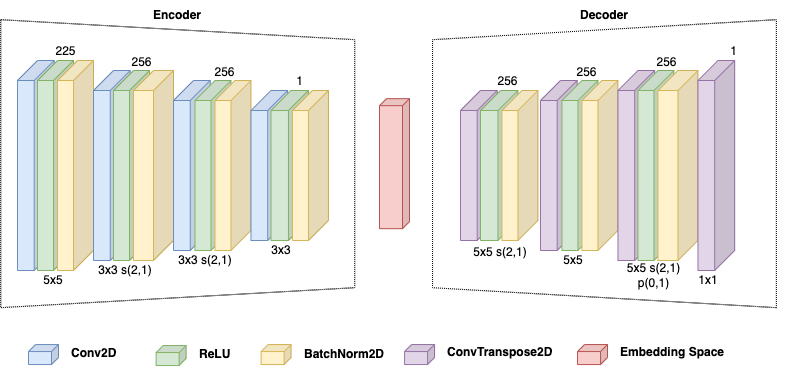
\includegraphics[width=\textwidth]{images/experiments/autoencoder_init.png}
\end{figure}

\subsubsection{Testing/Evaluation}
Regarding the evaluation of this first model, it has been tested out on the remaining 20\% of the small subset. These first experiments, consisted just of evaluating the outcome of the decoder, by passing single spectrograms through the network. By this, the ability of the network to recreate audio spectrograms got proven, which further on serves as a base for the next experiments. Regarding the final outcoming sounds, the original preserved phase information was reused to recreate audios.

\subsection{Spectrograms of signalframes as Input}
In the previous initial experiment, the samples from the NSynth dataset have been taken as a whole for the experiment. It has been mentioned, that all samples are 4 seconds long, but some contain padding in order to come to the 4 seconds. As those zero-paddings are then also part of the trained that, this could affect the behaviour but also the outcome of the model. If those zero-paddings would be left out, this leads to unequal long samples, which brings the problem with it, that they cannot be used for the model. Not used at all, as the network has a fixed size of neurons at the input, which means that the input has to be in a fixed shape. Furthermore this also means, that having a fixed size of 4 seconds, the input always has to be of 4 seconds, which is not desirable. Not at least, if the system should be used in real-time applications for audio synthesis, one cannot wait to have 4 seconds of a signal, to perform audio synthesis with it. Therefore it would be desirable to perform audio synthesis on smaller "frames or chunks" of an audio signal, respective spectrogram. 

\subsubsection{Pre-processing}
This leads, to the idea to take chunks or frames of audio data that get transformed into distinct spectrograms of same size. For a start the length of those frames, gets set to 500 ms. Furthermore it got chosen, that those frames are not consecutive, but have an overlap of 50\%. This should preserve the continuity of the signal \footnote{not sure if right}. Additionally those frames get multiplied with a window function, like it is used in the STFT. Similar to the window function used in the STFT, here a Hann-window is used.  Again as those trimmed signals all are differently long, they have to get padded to a multiple of the frame size respective hop-length. This ensures to have equally long chunks of the signal. As of the windowed frames, the first and last frame don't have overlapping parts at the beginning respective end. To overcome this issue, additional zeros get added there to form one frame on each side, to get there also an overlap. In combination, having the framed and windowed signal chunks, by overlapping each again with 50\% and adding the values, this would yield the original signal again. This gets especially helpful when reconstructing the final signal in the end. 

Having those framed and windowed signal chunks, the STFT gets applied on those, having the same configuration as in the first experiment. This then leads to have multiple spectrograms for the length of 500 ms with again a frequency resolution of 31,25 Hz. Again for the training and testing, additional to the log-mag data, the phase information, reference value and name of the sample including a number to identify the frame.

\subsubsection{Model and training}
The configuration of the model is rather similar to the one used in the first setting. It has the same amount of layers on each side, despite different strides, but also different kernel-sizes got applied. Again this one has been trained on 80\% of the \textit{keyboard\_synthetic} test dataset samples. Of course the significant difference here is, that now the input data are not whole spectrograms but overlapping frames. This also means, that the amount of data has increased. When collecting the spectrograms for the dataset, the names get shuffled, in order to not have the same order. In contrast, the single frames, don't get shuffled as well not during training. Again the training has been performed over 20 epochs on the local machine.

\subsubsection{Testing/Evaluation}
For the purpose of evaluating the test score this has been done with the remaining 20\% of the samples. To evaluate the ability of the autoencoder to reconstruct spectrograms, the whole samples are used including those from the training. Here the spectrograms are provided in the order as they appear. Having all reconstructed spectrograms, the inverse STFT got applied with the preserved phase information. Resulting in the frames corresponding to every single input note, those got overlapped and added (in their right order). By this procedure the signal with the original length could be obtained and further on evaluated auditorily. For results see chapter \ref{cha:Results}. 

A step for interpolating two different sources has not been investigated here, up to these experiments. Also the embedded space also has not been evaluated so far but will be subject of further experiments.

\section{Experiments single frequency vectors}
The above mentioned experiments, were a prove regarding the ability of convolutional autoencoders to recreate audio spectrograms. From this point on the experiments were done using the whole training dataset and also include audio synthesis. In the previous experiment the model is trained on frames of audio data which are 500ms long. Having the idea to synthesise audio with real-time input, this would mean that always a signal frame of 500ms has to be present, in order to have an input for the model. Therefore it is desirable to have an input that is as short as possible. In important note at this point is therefore, that spectrograms consist of frequency x time data. Each vector of the spectrogram along the time axis therefore represents a short frame of time. 

As mentioned before, when pre-processing is done on 16kHz sampled data with an n\_fft of 512, respective hop-length of 256, a time resolution of 16 ms is therefore present. Therefore the idea is to take those single frequency vectors, as input for the model. The shape therefore will be frequency x channels which in the case of the previous parameters is 256 x 1. With this idea, also the silence at the end of the signals can be omitted as just the frequency domain gets used for the models input. This therefore enables to take samples of different length in time. Throughout the experiment the value for the n\_fft got increased to 1024, as an increase of the models performance could be achieved (more on that in chapter \ref{cha:Results}). Increasing this parameter therefore means to decrease the time resolution, but increase the amount of frequency bins and thus having a better frequency resolution. Resulting in a number of 513 frequency bins (15,625 Hz/bin) and time resolution of 32ms per vector.


\subsubsection{Neural network}
As a consequence this means, that also a different model has to be used, as 2D-convolutions are no more suited. Therefore a model has been designed that uses 1D-convolutions. 1D-convolutions are performing the same calculations, with the difference of having just a 1-dimensional kernel. This one dimensional kernel therefore operates on the frequency axis and tries to extract important features. Equally to the 2D-convolutions they also apply the principle of channels. Regarding the channels, those also get expanded but then subsequently until the innermost layer reduced to 1 in order to form a single dimensional vector. Until the end again those channels get expanded but reduced again to 1 at the end to have the same shape as the input vector. In the following graphic (figure \ref{fig:cae_1D}), the structure and configuration of this autoencoder is depicted. 

 \begin{figure}[htb!]
	\caption{Deep 1D-convolutional autoencoder}
	\label{fig:cae_1D}
	\centering
	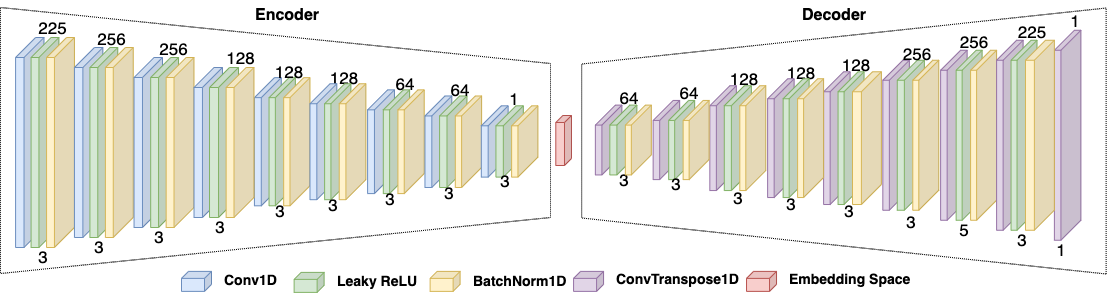
\includegraphics[width=\textwidth]{images/experiments/autoencoder_deep_1D.png}
\end{figure}

Here it can be seen, that in contrast to the one used in the initial experiment (see section \ref{sec:exp_init_experiment} figure \ref{fig:cae_2D_init}), leaky ReLU is used instead of normal ReLU. The use of the Leaky ReLU was also documented, in the work of \textit{Engel et al.} \cite{Engel2017} where it was used as activation function in the convolutional autoencoder. In the beginning for this experiment, normal ReLUs were used, but later on leaky ReLUs got applied and proven beneficial regarding model performance. This model also does not include, strides in the convolutional layers, which means, that the input does not get significantly downsampled towards the "bottleneck". One more notable difference is the depth of the network, as it has on each side 9 layers, resulting in a 18 layer network. Regarding the sublayers, also batch normalization gets applied, whereas it is also 1-dimensional, just as the convolutional layer. With all this configuration, the size of the embedding therefore would be 495x1x1. Throughout the experiment with 1D-convolutional networks, of course different configurations have been made, but this one worked out best. The results using this network can be seen later on in chapter \ref{cha:Results}.

\subsubsection{Training}
The training process for this experiment, differs in some major points from the previous ones. The main difference lies in the shape of the data. This can be concluded as here just the single frequency vectors, are used for this network and therefore the network itself has 1D-Convolutions as discussed before. Furthermore, this experiment was originally trained locally with the small subset like before, but later on access to a GPU-accelerated instance was made available. This GPU-instance, as discussed at the beginning of this chapter, enables to train complex ML-models with a large amount of data, over a long time. With this possibility, the training dataset can be utilized as this consists of several thousands of audio samples and would be too big to train locally. This does not mean, that the whole dataset was used all the time for training on this instance. With the progress of the project, several trainings with different amounts of data, could be made. Those are to be mentioned:

\begin{itemize}
    \item \textbf{Single Instrument}
    \item \textbf{Multiple Instruments (>=2)}
    \item \textbf{All Instruments}
\end{itemize}

Regarding the training performance, some interesting findings and observations could be made which get mentioned when showing the results. 

As here single frequency vectors are used, the process of creating a tensor and subsequently the dataset for the dataloader, is different. Here all spectrograms of the pre-defined and pre-processed dataset, were used, and the single frequency vectors get concatenated to form one big 3D array in the shape of amount x channels x frequency. To note the amount of channels here is also one in the input data. When experimenting with the training and its performance, also different strategies regarding shuffling got used. First on just the names of all samples got shuffled resulting in the instruments being mixed, but the frequency vectors were in the same order as in the spectrogram. This stays the same as after each epoch the data doesn't get shuffled. One more strategy that was found more successful, was also to shuffle the whole generated array, resulting in the frequency vectors of all instruments are mixed. Furthermore shuffling was also done after each epoch. The same strategies got also applied to the validation dataset, as from this point on also the validation dataset was considered. Not at least as more computational power was present from this point on. The most time, a batch-size of 32 was being used. 

Like discussed in chapter \ref{cha:Approach}, for the training also a validation step is needed. This validation was made using the validation dataset, which does not intersect with the training dataset. The validation process takes place in each epoch, after the training has been performed. This includes calculating of the train loss, back-propagating the error and optimizing the network. With this step, the network gets validated on data that has not been seen before, to prevent the network from overfitting. Introducing the validation step, also the scheduler to adapt the learning rate during the training gets applied here. Taking into account, that the network is rather complex and a huge amount of data has been used, the learning rate also has to be chosen adequately. Throughout this experiments, a small learning rate of $1e-7$ was chosen, as this led to a more stable training and better convergence. 

\subsubsection{Testing}
As described above, after each training, the current model state gets saved, those can be used for the testing and evaluation regarding synthesis. As having numerous states that got saved, the one with the lowest error score on the validation set gets taken for further steps. For the steps around testing and evaluation, the held-out test dataset gets used. This stage has been configured, to either take the whole test-dataset, a specific pitch, or a specific instrument source. By this technique its made possible to get the scores and therefore performance for certain instruments or pitch. 

\subsection{Experiments for Synthesis}
Having this kind of network that got trained on the training dataset, to reconstruct single frequency vectors, some experiments have been conducted for generating audio. As during the training the network learned how to reconstruct frequency vectors, one experiment is to examine the quality of the output for a single non-modified audio. Those are similar to the ones conducted, in first experiments above. Also by reconstructing just single notes those, the phase information was present, which enabled to apply the ISTFT. For a comparison also the Griffin-Lim algorithm got utilized.

As the main objective of this work is to examine the capability of creating novel sounds, from this point on in the project the interpolation step got introduced. With the interpolation step the encoded features in the embedded space of two instruments, get taken and value-wise interpolated. As it is known by this point, the encoder part of this network takes as input a vector of 513x1 and creates a lower-dimensional representation of it with the size of 495x1. Those representations, can be seen as the essential features, and got considered for the interpolation task. For this task, the frequency vectors of two instruments of probably the same pitch get passed through the network. Here the data does not get shuffled, as its important to produce the values in the same order as they come from the spectrograms. The output of the encoder for each instrument, gets concatenated to a 2D-array 495 x N where N is the number of encoded frequency vectors. To get a better idea of this concept, the next graphic (figure \ref{fig:exp_spec_emb_int_1D}) shows two spectrograms with the corresponding accumulated output of the encoder. 

 \begin{figure}[htb!]
	\caption{Input spectrograms with embeddings and interpolated embedding}
	\label{fig:exp_spec_emb_int_1D}
	\centering
	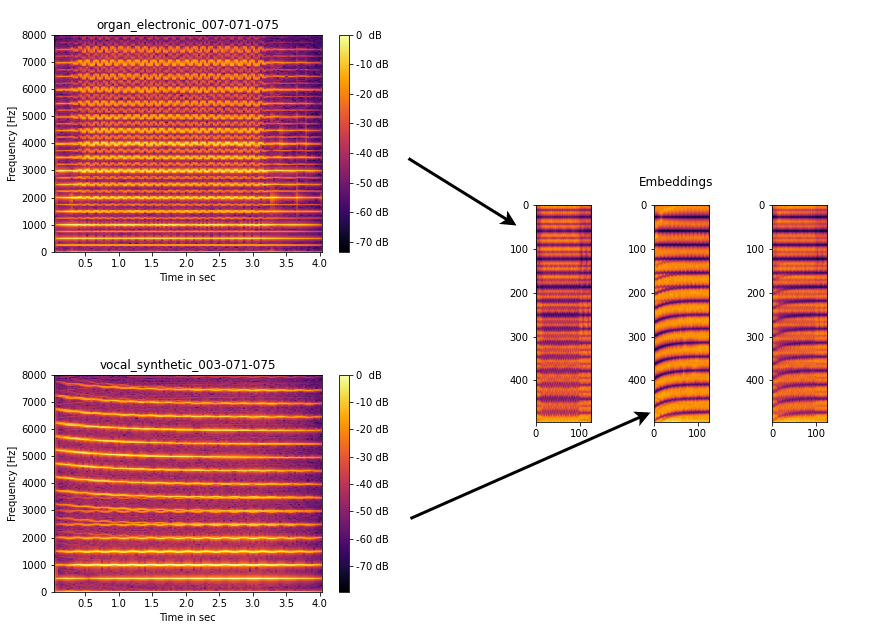
\includegraphics[width=\textwidth]{images/experiments/spec_to_emb.png}
\end{figure}

Having those two representations, interpolation gets performed. Like discussed in chapter \ref{cha:Approach}, along the x-axis each output vector of one sample gets interpolated with the corresponding output vector of the second sample. This process is also shown in figure \ref{fig:exp_spec_emb_int_1D} where the result of the interpolation process is shown. This process got applied equally for each subsequent experiments as the encoder output is always of the same shape, but more on that later on.
This interpolated vector gets subsequently passed through the decoer part which forms again frequency vectors of 513x1 which get accumulated to final spectrogram. This spectrogram then depicts the result of audio synthesis combining features of two different instruments.

Further on this spectrogram gets converted back to audio domain. As in this case no phase information is present, the Griffin-Lim algorithm \cite{Griffin1984} for phase estimation gets applied. By listening to the final sound, it should be possible to hear the characteristics of both instruments combined in this sound.

\section{Experiments with slices of spectrograms}
Based on the results and insights that could be gained with the previous experiments (see chapter \ref{cha:Results}) some more experiments were made. Not at least, to examine how different representations of the input data and as a consequence different model configurations influence the task of neural audio synthesis. For this case the following experiments in contrast work with 2D-representations as input. As 2D data there already have been the the initial experiments with whole spectrograms but also spectrograms based on frames of the audio signal. As a difference for the following experiments, the spectrograms have been taken, but sliced into overlapping chunks. The spectrograms taken in this experiment, got generated with the same configurations, as in the previous experiment (\texttt{n\_fft=1024}, \texttt{hop\_length=512}). The idea to use chunks of spectrograms as input, arose to improve the models performance with regard to synthesis and recreation of spectrograms. As by using single frequency vectors, there is just the freuqency information present and no information about its change over time. As a theory to also incorporate the temporal axis as input, important information about the temporal frequency changes could be captured. Those frequency changes could deliver more important characteristics of the samples that could be extracted. As not the whole spectrograms should be used as input, chunks of them are favorable, to keep the input as small as possible. Therefore the choice has been made to take three consecutive frequency vectors to form a frame with the shape of (513x3). Throughout the experiments it has been tried out to either take the frames subsequently or overlapping, leading to the preference in taking the latter. The overlap has chosen to be always 2 vectors from the preceding frame. 

For demonstration, let there be a spectrogrogram $spec=[v_0, v_1, v_2, v_3, v_4, v_5, ... v_n]$ of length $n$ where $v_i$ is the frequency vector at index $i$. This results in an array of $frames=[[v_1, v_2, v_3], [v_2, v_3, v_4], [v_3, v_4, v_5] ... [v_{n-3}, v_{n-2}, v_{n-1}], [v_{n-2}, v_{n-1}, v_n]]$. The idea behind this overlap is to capture every change or time-pattern in the source spectrogram. This technique also has the advantage that all the silence of the source spectrograms can be cut away, allowing to use differently long spectrograms as input. A positive side-effect here is also, to gain more amount of data, on which the model can be trained on. As the models output are also overlapping frames, to reconstruct the final spectrogram and audio, this has also to be considered, but more on that later on. Again when creating the tensor and dataset, the spectrograms get taken in a random order. At first the resulting frames of the training set, don't get shuffled. Later on during the training, the frames in the batches, which again are of size 32, get shuffled like in previous examples. The same happens to the validation dataset, while it also gets shuffled initially but also after each epoch. An important note is that for the training and validation the whole dataset got used all the time. 

\subsubsection{Neural Network}
As again input data in a 2D-shape was used for these experiments, the model again has to be adapted. Instead of 1D-convolutions and 1D-batch-normalization again, 2D-convolutions and 2D-batch-normalization has been used. Also in contrast to the previous network, a normal ReLU activation has been used. These experiments incorporate different model configurations whereas a special focus has been given to the amount of striding and thus input compression. Here it should get evaluated, how more compression and thus a smaller latent space, influences the quality of the decoder output and further on of the generated audio. Both in terms of single note reconstruction and interpolation based synthesis. The following figure (\ref{fig:exp_2D_cae}) shows, the basic network structure for this kind of experiments.

 \begin{figure}[htb!]
	\caption{2D-convolutional autoencoder}
	\label{fig:exp_2D_cae}
	\centering
	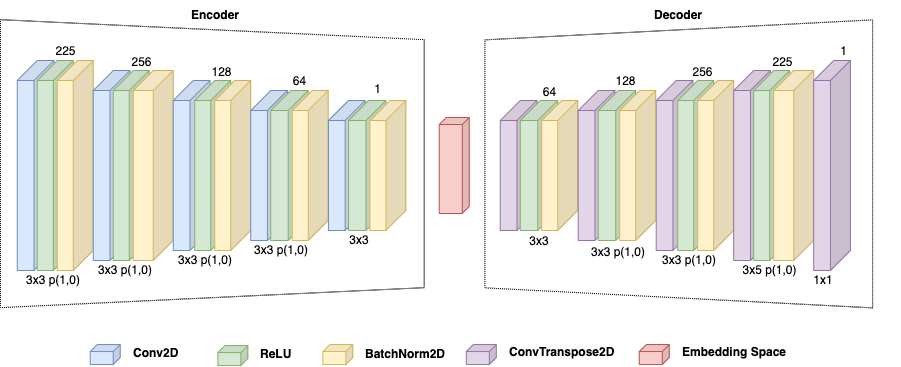
\includegraphics[width=\textwidth]{images/experiments/autoencoder_2D.png}
\end{figure}

This network is not as deep as the one used in the previous experiment as it consists of 5 layers on each side (10 in total). As the input is of size 513x3, the network has to use a padding along the time-axis. If no padding would be applied, just one time a kernel of 3x3 could be applied. Thus 5 times a 3x3 kernel could be applied with the last layer having no padding. This results in a single 1D-vector in the embedded space. In the decoder part, padding also has to be applied to come again to the same dimensionality in the end. As previously said, these experiments should give an insight on how the striding and thus the size of the embedding influences the performance and quality of the output. Choosing more strides and a smaller embedding, the network has to learn to extract more efficient encodings, from which it can reconstruct the input data. Thus by choosing a small embedding size, the network should learn to extract the most important features of the input. Therefore the size is also of significance regarding the audio synthesis task by interpolating the embeddings. In the following table (\ref{tab:exp_2D_strides}), the different configurations regarding the striding are shown. 


\begin{table}[htb!]
    \centering
    \begin{tabular}{|c|c|c|c|}
        \hline
         &\textbf{Encoder}&\textbf{Embedding-size}&\textbf{Decoder} \\
         \hline
        \textbf{Single Stride} & e2 & 250 & d4 \\
        \hline
        \textbf{Double Stride} & e2, e4 & 124 & d2, d4 \\
        \hline
        \textbf{Triple Stride} & e2, e3, e5 & 62 & d1, d3, d4 \\
        \hline
    \end{tabular}
    \caption{Setting of stridings in network}
    \label{tab:exp_2D_strides}
\end{table}

To explain, each row represents a network configuration, that either uses one, two or three times a striding of (1,2) on each side of the network. As of the shape of the input, striding just can be applied on the frequency axis. The columns with the names "Encoder" and "Decoder" show the respective layers, where the stride got applied. For example e2 is the second layer in the Encoder and d4 the fourth layer in the decoder. The center column called "Embedding-size" explains the size of the embedded space vector. By having these model configurations, interesting findings and results could be obtained. 

\subsection{Audio synthesis}
In the previous experiment with the 1D-convolutional network, the interpolation step has been introduced. This step gets also applied with this network. As the embedded space vector also has the shape of a 1D-vector, the interpolation procedure here is exactly the same. 

\subsubsection{Analysis of the embedded space}
As with neural audio synthesis novel interesting sounds should get generated, it is also of interest to find interesting combinations for the interpolation. Combined with the fact, that the embeddings contain the extracted features/characteristics of a sound, those can get utilized for this task. It therefore has been implemented to take the output of the encoder of several notes (e.g. from the same pitch) and compute the correlation coefficients between those. The result gets depicted in a correlation matrix to see which samples have the lowest correlation coefficients. Low correlation coefficients between two data samples mean that those have little similarities and thus different characteristics. By taking those embeddings with the lowest correlation coefficients and interpolate them, interesting novel sounds can be generated. More on that later in chapter \ref{cha:Results}.

\subsection{Reconstruction and post-processing}
As the shape of the output of the network is the same as of the input of the network, this has to be considered when recreating the spectrogram. The output therefore are also again frames of 3 that have to get overlapped. During the experiments different strategies have been tried out, whereas it got preferred to average the overlapping parts of the output frames, in order to form the final spectrogram.

When having the final spectrograms, some further experiments regarding the improvement of the sound quality have been carried out. In this case this includes to correct the frequency bands of the output. With this technique important properties of the sound like the transient or impulse (e.g. guitar stroke) should get preserved. For this task in advance the energy-values of the frequencies get summed up for each frequency vector of the original audio spectrograms. This gets also done for the output spectrogram and its frequency vectors, after converting from db to energy. By comparing those sums with the corresponding values of the input spectrogram, a factor can be calculated. This factor then gets multiplied with the corresponding output frequency vector in order to have the same amount of energy present in the output spectrogram. If the output spectrogram was generated by an interpolated embedding, the energy sums of the input samples get taken and averaged. This averaged values then get taken as a reference to correct the energy. By performing the inverse STFT or Griffin-Lim algorithm, the resultig audio sample should therefore also have a corrected amplitude and thus improved sound. Regarding the results, those get as well discussed later on in the thesis.


\section{Experiments with mel-scale}
Up to this point, the experiments have all been conducted on log-magnitude spectrograms. Those spectrograms depict the frequency energies on a linear scale with a certain resolution (e.g. $[0 Hz, 15.625 Hz, 31.25 Hz ... 8000 Hz]$). Those spectrograms have been computed of dataset consisting of musical notes. Those notes can be grouped into musical intervals describing the distance of a note to another, whereas the interval of an octave would be a doubling in frequency. As an example the note \textit{a'} has a frequency of 440Hz (if perfect sine), whereas its octave on top would be an \textit{a''} with 440Hz. If going an octave down it would result in 220Hz having an \textit{a} (to be continued \textit{A} 110Hz, \textit{A'} 55Hz, ...). This also means that the higher the note gets, the larger the distance in Hz and the lower it gets, the less distance in Hz between the notes. Having this principle in mind one can come to the conclusion that having a linear scale like in log-magnitude spectrograms, the resolution with lower notes is worse then with higher notes. With a look onto machine learning and neural networks, this also means, that there is less data available to train on for low notes.
Keeping this in mind, the choice has been made to make comparative experiments based on a different scale, which is called mel-scale \cite{stevens1937scale}. This scale can be seen as a compressed form of a spectrogram. This scale is an empirical scale that is based on the human auditory perception. This means that humans percept low frequencies louder and with a greater resolution then with higher notes. Mapped on a scale this means that the on mel-scale, in contrast to magnitude, lower notes have a greater distance between them. The opposite applies to the higher notes as there the distance gets less. This means that with this scale lower notes can be better differentiated and thus get more emphasized then with Hertz. Even though that this scale is based on observations it gets proven to be beneficial regarding machine learning-tasks. Not at least as several approaches, that also have been mentioned in related work applied this scale for their audio synthesis task. Furthermore this scale can also be seen as a compressed form of a spectrogram containing the most significant properties. 

\subsubsection{Pre-processing}
The pro-processing step does not really differ from the ones performed in previous experiments. A difference here is in order to obtain spectrograms with the mel-scale to call the \textit{librosa} function \texttt{librosa.feature.melspectrogram} which takes as input a pre-computed STFT-spectrogram. Throughout this experiment the spectrograms created with an n\_fft of 1024 and hop\_length of 512 have been taken to be converted to mel-spectrograms. Having the mel-sepctrograms the same steps as with log-magnitude get performed (db conversion, preserving the power reference,...). Also for the model-training, frames of 3 vectors of the mel-spectrogram get taken as input for the model. In the next figure a mel-spectrogram with its corresponding log-magnitude spectrogram can be seen.


